\chapter{Implementierung}
Die Implementierung der Explorationskomponente besteht aus drei Hauptbestandteilen, die jeweils als separates Java-Projekt umgesetzt wurden. Im weiteren Verlauf werden diese Java-Projekte als Module bezeichnet.
\\\\
In Abbildung \ref{fig_arch} ist die Architektur der Explorationskomponente aufgeführt. Die das Modul \emph{DesiredComponentSourcerer} stellt eine Schnittstelle nach Außen bereit, über die die Explorationskomponenten in ein beliebiges Projekt eingebunden werden kann. Weiterhin ist das Modul \emph{DesiredComponentSourcerer} von den Modulen \emph{ComponentTester} und \emph{SignatureMatching} abhängig, die selbst keine Abhängigkeiten zueinander haben.
\\\\
Darüber hinaus, werden folgende externe Bibliotheken verwendet:
\begin{itemize}
\item easymock 3.0 \cite{easymock}
\item cglib 3.3.0 \cite{cglib}
\item objenesis 3.1 \cite{objenesis}
\item junit 4.13.0 \cite{junit}
\end{itemize}
Auf die konkrete Verwendung der externen Bibliotheken wird in den detaillierteren Beschreibungen der einzelnen Module in den folgenden Abschnitten eingegangen. Im Anschluss an die Beschreibung der Module wird auf die Nutzung der Schnittstelle zur Einbindung der Explorationskomponente in beliebige Java-Projekt eingegangen.
\section{Modul: SignatureMatching}
\begin{figure}
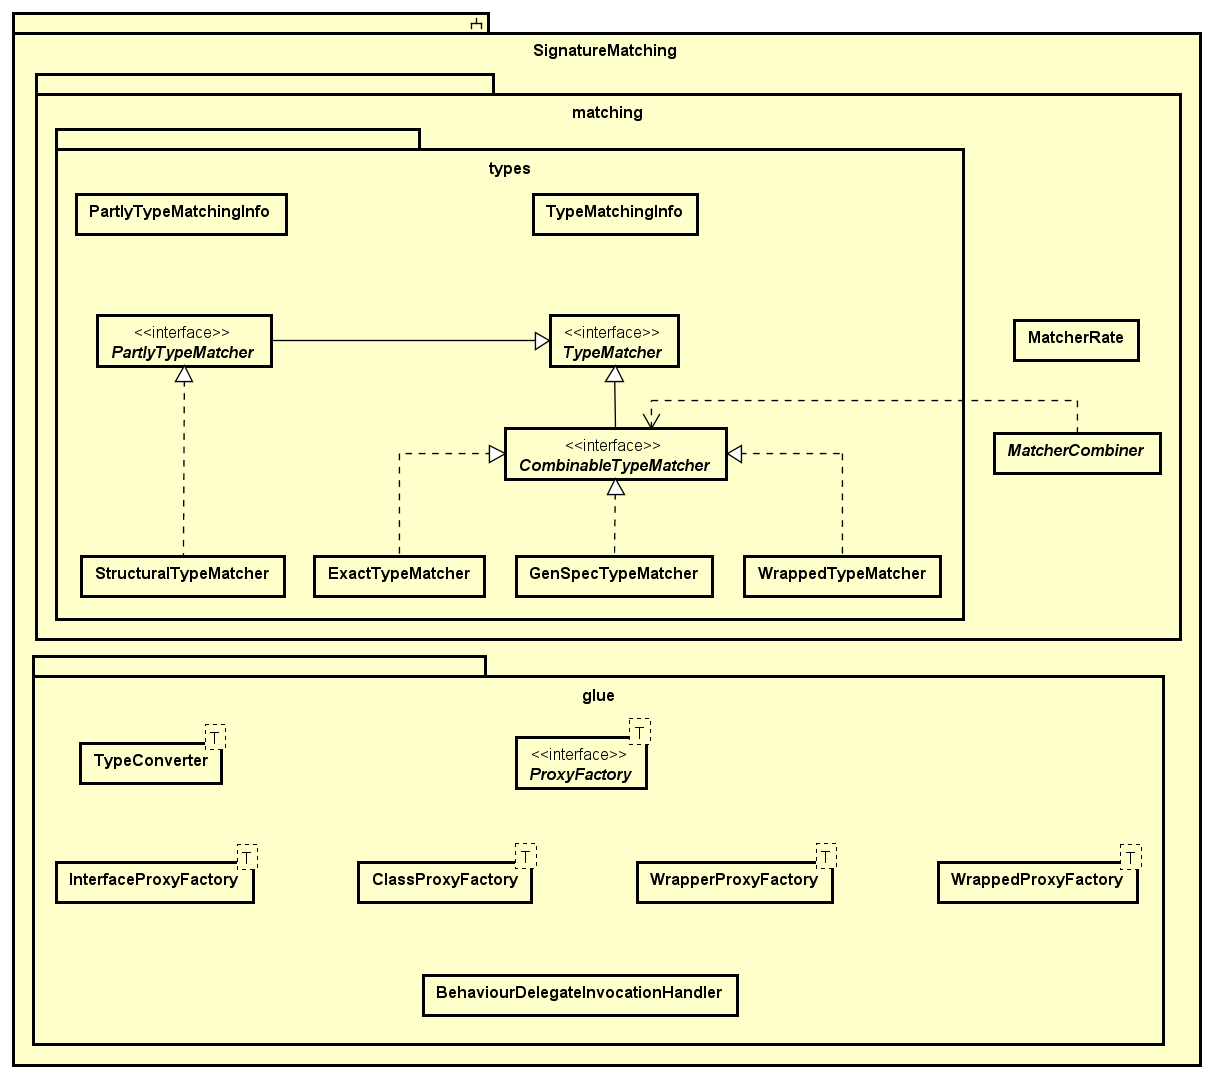
\includegraphics[scale=0.5]{cd_SigMa.png}
\caption{Modul: SignatureMatching}
\label{fig_cdSigMa}
\end{figure}
\begin{figure}
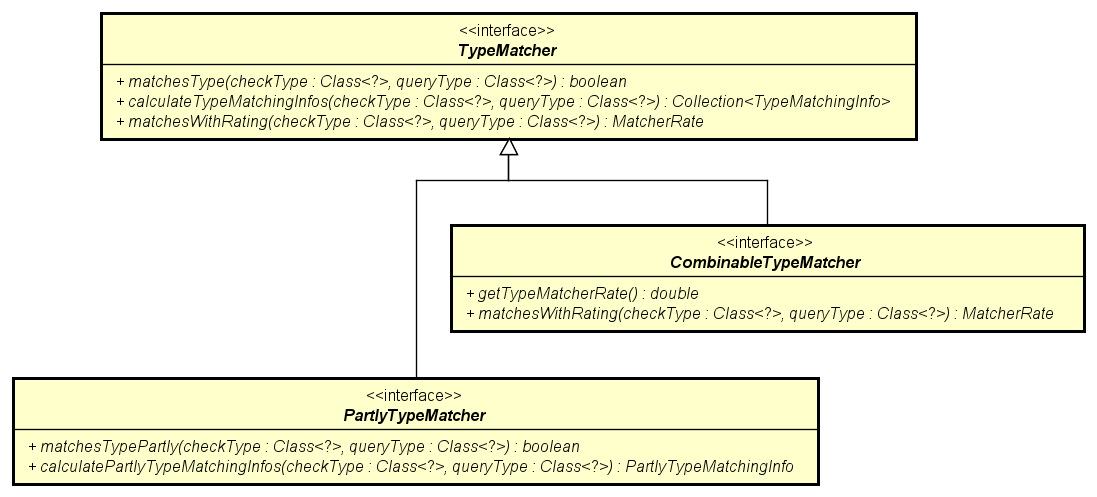
\includegraphics[scale=0.5]{cd_TypeMatcher.png}
\caption{TypeMatcher-Interfaces}
\label{fig_cdTypeMatcher}
\end{figure}
In diesem Modul befinden sich zum Einen die Implementierungen der Matcher, die in Abschnitt \ref{sec_matcher} formal beschrieben wurden und zum Anderen die Implementierung der Generatoren für die Proxies. In Abbildung \ref{fig_cdSigMa) sind die wichtigsten Klassen und Interfaces dieses Moduls mit ihren Abhängigkeiten zueinander aufgeführt. Die Matcher befinden sich dabei im Package \emph{matching} und die Generatoren für die Proxies im Package \emph{glue}.
\\\\
Die in Abschnitt \ref{sec_matcher} beschriebenen Matcher wurden teilweise in einer Klasse zusammengefasst. Tabelle \ref{tab_matcher2impl} zeigt die Zuordnung von Matchern zu den jeweiligen Klassen.
\begin{table}[h!]
\centering
\begin{tabular}{|l|l|}
\hline
\hline
\textbf{Matcher} & \textbf{Implementierung (Klasse)} \\
\hline
ExactTypeMatcher & $\texttt{ExactTypeMatcher}$ \\
\hline
GenTypeMatcher & $\texttt{GenSpecTypeMatcher}$ \\
\hline
SpecTypeMatcher & $\texttt{GenSpecTypeMatcher}$ \\
\hline
ContentTypeMatcher & $\texttt{WrappedTypeMatcher}$ \\
\hline
ContainerTypeMatcher & $\texttt{WrappedTypeMatcher}$ \\
\hline
StructuralTypeMatcher & $\texttt{StructuralTypeMatcher}$ \\
\hline
\hline
\end{tabular}
\caption{Zuordnung der Matcher zu den Klassen, in denen sie implementiert sind}
\end{table}\label{tab_matcher2impl}
\noindent
Die Klasse $\texttt{StructuralTypeMatcher}$ nimmt dabei eine Sonderstellung ein. Dies ist daran zu erkennen, dass dieser nicht das Interface $\texttt{TypeMatcher}$ implementiert. Dies wird damit begründet, dass es sich bei diesem Matcher um den Einstiegspunkt der strukturellen Evaluation handelt. Analog zum StructuralTypeMatcher aus Abschnitt \ref{sec_matcher} wird in der Klasse $\texttt{StructuralTypeMatcher}$ nämlich auf die anderen Matcher bzw. Matcher-Implementierungen zugegriffen, was in Abbildung \ref{fig_cdSigMa) durch die Komposition zwischen der Klasse $\texttt{StructuralTypeMatcher}$ und dem Interface $\texttt{TypeMatcher}$ angedeutet wird.
\\\\
Die übrigen Matcher implementieren das Interface $\texttt{TypeMatcher}$ und können über die Methoden aus der Klasse $\texttt{MatcherCombinator}$ miteinander kombiniert werden\footnote{Ein Beispiel für die Kombination von Matchern ist im Anhang \ref{app_matchercombination} zu finden.}. 
%TODO ANHANG: Kombination (siehe unten)
So kann eine Kombination mehrerer $\texttt{TypeMatcher}$, die wiederum von Type $\texttt{TypeMatcher}$ ist, in der Klasse $\texttt{StructuralTypeMatcher}$ verwendet werden. Die konkrete $\texttt{TypeMatcher}$-Kombination, die im $\texttt{StructuralTypeMatcher}$ instanziiert wird, orientiert sich an den Ausführungen in Abschnitt \ref{sec_matcher}. Es ist aber zu erwähnen, dass die Verwendung weitere Matcher, die in dieser Arbeit nicht definiert wurden, denkbar ist. Eine solche Erweiterung ließe sich leicht in dieses Modul über die Implementierung des Interfaces $\texttt{TypeMatcher}$ und den $\texttt{MatcherCombiner}$ bewerkstelligen.
\\\\
Alle Matcher-Implementierungen bieten die Möglichkeit, zu ermitteln, ob ein Matching zwischen zwei Typen besteht. Dies erfolgt jeweils über die Methode $\texttt{matchesType}$. Darüber hinaus werden über die Methoden $\texttt{calculateMatchingInfos}$ (in den Implementierung des Interface $\texttt{TypeMatcher}$) bzw. $\texttt{calculateMatchingInfo}$ (in der Klasse $\texttt{StructuralTypeMatcher}$) Informationen bzgl. der Methodendelegationen zwischen den beiden gemachten Typen ermittelt. Diese Informationen werden in einem Objekt der Klasse $\texttt{SingleMatchingInfo}$ bzw. $\texttt{MatchingInfo}$ zusammengetragen. 
\\\\
Diese beiden Klassen unterscheiden sich lediglich bzgl. der Anzahl von Methoden, an denen die aufgerufene Methode des \emph{Source}-Typ (Attribut $\texttt{source}$) delegiert werden kann (siehe Attribut: $\texttt{methodDelegationSupplier}$). Während ein Objekt der Klasse $\texttt{MatchingInfo}$ mehrere Delegationsmethoden zu einer aufgerufenen Methoden enthalten kann, darf ein Objekt der Klasse $\texttt{SingleMatchingInfo}$ lediglich eine Delegationsmethode zu einer aufgerufenen Methode enthalten (vgl. auch Abschnitt \ref{sec_matcher}). Zusätzlich zu erwähnen ist, dass die Informationen über die Delegationsmethoden aus einer $\texttt{MatchingInfo}$ über in einem $\texttt{MethodSupplier}$ überliefert wird.
\\\\
Eine Instanz der Klasse $\texttt{MethodSupplier}$ enthält zum Einen ein $\texttt{MatcherRating}$ welches Informationen bzgl. des in Abschnitt skjfdkhaksg beschriebenen Matcher-Ratings beinhaltet. Zum Anderen werden im Attribut $\texttt{methodMatchingInfo}$ in einem Objekt der Klasse $\texttt{MethodMatchingInfo}$ die Informationen bzgl. der Delegation der aufgerufenen Methode an die Delegationsmethode hinterlegt. 
\\\\
Bezüglich der Klasse $\texttt{SingleMatchingInfo}$ ist noch das Attribut $\texttt{proxyFactoryCreator}$ zu beschreiben. Darin werden Informationen bzgl. der strukturellen Verbindung von zwischen den gematchten Typen gehalten. Für den \emph{ExactTypeMatcher}, den \emph{GenTypeMatcher} und den \emph{SpecTypeMatcher} wird dabei ein $\texttt{ProxyFactoryCreator}$ erzeugt, der in der Lage ist, eine $\texttt{ProxyFactory}$ für Typen zu erzeugen, die in einer nominalen Beziehung \footnote{Identität, Generalisierung, Spezialisierung} stehen. Für den \emph{ContentTypeMatcher} und den \emph{ContainedTypeMatcher} hingegen, wird ein $\texttt{ProxyFactoryCreator}$ erzeugt, der in der Lage ist, eine $\texttt{ProxyFactory}$ für Typen zu erzeugen, bei denen der eine Typ ein Attribut von Typ des anderen enthält. Die erzeugten Objekte vom Typ $\texttt{ProxyFactory}$ werden bei der Generierung der Proxies unter der Zuhilfenahme der Bibliotheken \emph{cglib} und \emph{objenesis} verwendet\footnote{Diese beiden Frameworks wurden verwendet, da die Erzeugung der Proxies mit ihnen komfortabler ist, als mit den Mitteln die das JKD zur Verfügung steht. Dies gilt insbesondere für die Erzeugung von Proxies für Klassen, die mit dem Schlüsselwort $\texttt{final}$ versehen sind.}.
\\\
Der $\texttt{ProxyFactoryCreator}$ stellt damit eines der Bindeglieder zwischen der Package \emph{matching} und dem Package \emph{glue} innerhalb des Moduls her. Das zweite Artefakt, welches als Bindeglied fungiert, ist die oben bereits erwähnt Klasse $\texttt{MethodMatchingInfo}$.
\\\\
Ein Objekt der Klasse $\texttt{MethodMatchingInfo}$ enthält in den Attributen $\texttt{source}$ und $\texttt{target}$ je eine Methode. Dabei ist im Attribut $\texttt{source}$ die aufgerufene Methode der Methoden-Delegation und im Attribut $\texttt{target}$ die Delegationsmethode enthalten. Darüber hinaus wird im Attribut $\texttt{returnTypeMatchingInfo}$ ein Objekt der Klasse $\texttt{ModuleMatchingInfo}$ gehalten , welches alle notwendigen Informationen für das Erzeugen eines Proxies des Rückgabetyp der aufgerufenen Methode aus dem Rückgabetyp der Delegationsmethode. Analog dazu wird im Attribut $\texttt{argumentTypeMatchingInfos}$ eine Map, bestehend aus weiteren Objekten der Klasse $\texttt{ModuleMatchingInfo}$ und jeweils einem Objekt der Klasse $\texttt{ParamPosition}$, gehalten. Diese Map enthält alle notwendigen Information für das Erzeugen eines Proxies für die Parametertypen der Delegationsmethoden aus den Parametertypen der aufgerufenen Methode, sowie der Anpassung der Übergabeposition bei der Delegation der aufgerufenen Methode (siehe auch Abschnitt \ref{sec:proxygram}).
\\\\
Um die Methoden-Delegationen zu koordieren, wird bei der Erzeugung des Proxies in der jeweiligen $\texttt{ProxyFactory}$ für das Proxy-Objekt ein $\texttt{InvocationHandler}$ instanziiert (vgl. \cite{invocationhandler}. Dieses Interface wird im \emph{glue}-Package durch die Klasse $\texttt{BehaviourDelegateInvocationHandler}$ implementiert, in der letztendlich die Koordination der Methoden-Delegationen auf Basis der jeweiligen $\texttt{MethodMatchingInfo}$ spezifiziert ist.
\\\\
Um einen Proxy basierend auf dem Matching zweier Typen zu erzeugen steht die Klasse $\texttt{TypeConverter}$ zur Verfügung. Die Zugriffe innerhalb des Packages \emph{glue} als auch die Zugriff von außerhalb benötigen jeweils ein Objekt der Klasse $\texttt{ConvertableBundle}$. Diese Klasse beschreibt eine Kombination mehrerer Objekte vom Typ $\texttt{ConvertableComponent}$, die als Delegationsziele des zu erzeugenden Proxy-Objektes fungieren sollen. Ein Objekt der Klasse $\texttt{ConvertableComponent}$ enthält eine Liste von Objekten vom Typ $\texttt{ModuleMatchingInfo}$, die wie bereits erwähnt beschreiben, am welche Methode die Delegation erfolgen soll. Das Objekt im Attribut $\texttt{convertableObject}$ der $\texttt{ModuleMatchingInfo}$ beinhaltet das Objekt, auf dem die Delegationsmethode aufgerufen werden soll.

%TODO ANHANG: Kombination (siehe unten)
%Die Matcher-Klassen $\texttt{ExactTypeMatcher}$, $\texttt{GenSpecTypeMatcher}$ und $\texttt{WrappedTypeMatcher}$ implementieren auch das von $\texttt{TypeMatcher}$ erbende Interfaces $\texttt{CombinalbeTypeMatcher}$. Klassen, die dieses Interface implementieren können über die Klasse $\texttt{MatcherCombiner}$ zu einem neuen $\texttt{TypeMatcher}$-Objekt kombiniert werden. Ein solcher kombinierte $\texttt{TypeMatcher}$ versucht beim Aufruf der Methode $\texttt{matchesType(S,T)}$ die beiden Typen $S$ und $T$ über einen der kombinierten Matcher zu matchen. Abbildung \ref{sd_matchercombiner} zeigt das Sequenzdiagramm für diesen Aufruf. Dabei liefert die Methode $\texttt{getSortedMatcher}$ eine sortiert Liste der kombinierten Matcher. Die Sortierung wird aufsteigend entsprechend dem Matcherrating der kombinierten Matcher vorgenommen.
%\begin{figure}
%\end{figure}\label{sd_matchercombiner}
%\noindent
%Darüber hinaus gibt es noch das von $\texttt{TypeMatcher}$ erbende Interface $\texttt{PartlyTypeMatcher}$. Dieses Interface wird nur von dem $\texttt{StructuralTypeMatcher}$ implementiert, welcher u.a. als Schnittstelle zwischen dem Modul \emph{SignatureMatching} und \emph{DesiredComponentSourcerer} fungiert. Wie der Name des Interfaces bereits impliziert, bieten die Implementierungen des Interfaces $\texttt{PartlyTypeMatcher}$ die Möglichkeit, zwei Typen nur teilweise zu Matchen. Das bildet die Grundlage für die Ermittlung der Typen, aus denen die Proxies für die semantische Evaluation erzeugt werden können (vgl. Abschnitt \ref{sec_ergStructEval}). So stellen die Objekte, die über die Methode $\texttt{calculatePartlyTypeMatchingInfos}$ erzeugten wurden, auf formaler Ebene die Elemente der Mengen, die in Abschnitt \ref{sec_ergStructEval} über Funktion $\texttt{cover}$ beschrieben wurden, dar.

\section{Modul: ComponentTester}
Dieses Modul ist für die Definition und Ausführung der vordefinierten Tests zuständig. Dabei sei davon auszugehen, dass ein required Typ $R$ in Form eines Interfaces existiert. Um Tests für $R$ zu definieren, können eine oder mehrere Testklassen implementiert werden. Die Testklassen werden dabei in dem Interface $R$ über das Attribut $\texttt{testClasses}$ der Annotation $\texttt{RequiredTypeTestReference}$ angegeben (siehe Abbildung \ref{fig_cdCompTester} Package: \emph{API}). Ein Beispiel für die Deklaration eines required Typ in Form eines Java-Interfaces und den dazugehörigen Testklassen ist im Anhang zu finden.
\\\\
Damit die Testmethoden in den Testklassen, den in Abschnitt \ref{sec_testanforderungen} beschriebenen Eigenschaften genügen und durch das ComponentTester-Modul ausfindig gemacht werden können, stehen mehrere Artefakte in dem API- und dem SPI-Package des ComponentTester-Moduls bereit (siehe Abbildung \ref{fig_cdCompTester}).
\\\\
So muss jede Testklasse eine Methode bereitstellen, über die ein Objekt vom Typ $R$ in die Instanz der Testklasse injiziert werden kann. Diese Methode wird von dem ComponentTester-Modul über die Annotation $\texttt{RequiredTypeInstanceSetter}$ gefunden. Von daher muss die Methode mit eben dieser Annotation markiert werden.
\begin{figure}
\centering
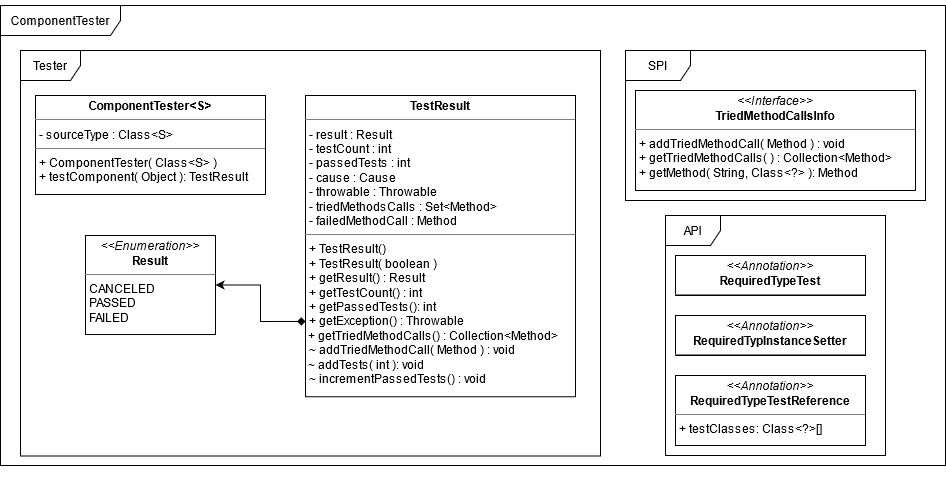
\includegraphics[scale=0.5]{pics/cd_ComponentTester.png}
\caption{Modul: ComponentTester}
\label{fig_cdCompTester}
\end{figure}
\\\\
Die Testmethoden müssen von der Sichtbarkeit her öffentlich ($\texttt{public}$) sein. Weiterhin dürfen die Testmethoden keine Parameter erwarten und müssen mit der Annotation $\texttt{RequiredTypeTest}$ markiert sein. Die Erwartungen innerhalb der Testmethoden müssen über die in JUnit 4 zur Verfügung stehenden Methoden aus der Klasse $\texttt{Assert}$ (vgl. \cite{junit_api}) deklariert werden. Testdaten, die für alle Testmethoden innerhalb einer Testklasse zur Verfügung stehen sollen, können diese innerhalb von Methoden erzeugt werden, die über die in JUnit 4 bereitgestellten Annotationen $\texttt{Before}$ und $\texttt{After}$ (vgl. \cite{junit_api}) versehen werden.
\\\\
Um die Reihenfolge der versuchten Aufrufe der Methoden, die von $R$ angeboten werden, zu verwalten, muss die Testklasse das Interface $\texttt{TriedMethodCallsInfo}$ implementieren (siehe Abbildung \ref{fig_cdCompTester} Package: \emph{SPI}). Dadurch wird die Implementierung der Methoden $\texttt{addTriedMethodCall}$ und $\texttt{getTriedMethodCalls}$ erzwungen. Die Methode $\texttt{getMethod}$ kann mit der default-Implementierung übernommen werden, sofern die in $R$ deklarierten Methoden über den Namen identifiziert werden können.
\\\\
Die Implementierung der Methoden $\texttt{addTriedMethodCall}$ und $\texttt{getTriedMethodCalls}$ hat so zu erfolgen, dass bei einem Aufruf der Methode $\texttt{addTriedMethodCall}$ der übergebene Parameter an eine Liste angefügt wird. Der Aufruf der Methode $\texttt{getTriedMethodCalls}$ liefert eben diese Liste als Rückgabewert. Weiterhin ist sicherzustellen, dass vor dem Aufruf einer Methode $m$ aus $R$ die Methode $\texttt{addTriedMethodCall}$ mit $m$ als Parameter aufgerufen wird. Im Anhang ist ein Beispiel für die korrekte Implementierung einer Testklasse zu finden.
\\\\
Der Test eines Proxies für $R$ wird über eine Instanz der Klasse $\texttt{ComponentTester}$ angestoßen (siehe Abbildung \ref{fig_cdCompTester} Package: \emph{Tester}). In Abhängigkeit der in $R$ deklarierten Testklassen werden alle darin befindlichen Testmethoden durchgeführt, bis einer dieser Testfälle fehlschlägt. Der Aufrufer erhält dabei ein der Klasse $\texttt{TestResult}$ zurück (siehe Abbildung \ref{fig_cdCompTester}). In diesem Objekt sind die für die Auswertung des Testergebnisses relevanten Informationen vorhanden, auf die die Heuristiken \emph{PTTF} (siehe Abschnitt \ref{sec_pttf}) und \emph{BL\_NMC} (siehe Abschnitt \ref{sec_bl_nmc}) angewiesen sind.
\section{Modul: DesiredComponentSourcerer}
In diesem Modul wird die Exploration koordiniert. Zum Starten der Exploration für ein \emph{desired Interface} muss zuerst eine Instanz der Klasse $\texttt{DesiredComponentFinder}$ erzeugt werden (genannt: \emph{Finder}). Dies erfolgt über einen Konstruktor, der ein Objekt der Klasse $\texttt{DesiredComponentFinderConfig}$ (genannt: \emph{Konfig}) erwartet (siehe Abbildung \ref{cd_finderCreation}). 
\begin{figure}[h!]
\centering
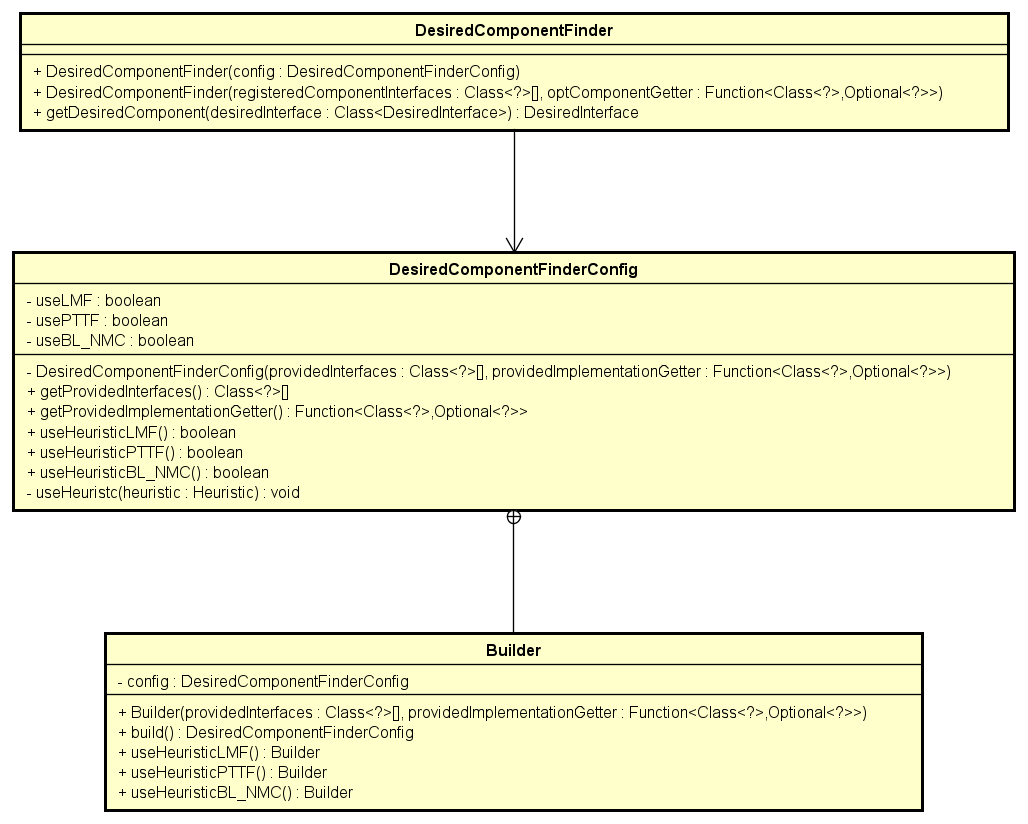
\includegraphics[scale=0.5]{cd_finderCreation.png}
\caption{Schnittstellen des Moduls: DesiredComponentSourcerer}
\label{cd_finderCreation}
\end{figure}
\noindent
Die Erzeugung einer solchen \emph{Konfig} erfolgt über einen Builder. Dabei müssen zum Einen die Angabe aller provided Typen in Form einer Liste von Interfaces. Zum Anderen wird eine Funktion ($\texttt{java.util.Function}$) gefordert, über die die Implementierungen der im Parameter übergebenen Interfaces ermittelt werden können.
\\\\
Zum Zweck der gezielten Evaluation der Heuristiken in Kapitel \ref{chap_evaluation} kann über die \emph{Konfig} gesteuert werden, welche der in Abschnitt \ref{sec_heuristics} beschriebenen Heuristiken bei der Exploration verwendet werden sollen. Dies erfolgt über die in Abbildung \ref{cd_finderCreation} ersichtlichen Methoden mit den Präfix $\texttt{useHeuristic*}$.
\\\\
Die Exploration wird nach der Erzeugung des \emph{Finders} über den Aufruf der Methode $\texttt{getDesiredComponent}$ mit der Übergabe des \emph{desired Interface} $R$ als Parameter. Im Anschluss wird die syntaktische Evaluation für alle \emph{provided Interfaces} durchgeführt. Auf formaler ebene gleicht dieser Schritt der Ausführung der Funktion $\mathit{cover(R,L)}$, wobei die in $L$ befindlichen \emph{provided Typen} auf die an der \emph{Finder} übergebenen \emph{provided Interfaces} beschränkt sind.
\\\\
Hierzu wird ein Objekt vom $\texttt{StructuralTypeMatcher}$ aus dem \emph{SignatureMatching}-Modul verwendet\footnote{Dieses Objekt wird beim Instanziieren des \emph{Finders} erzeugt.} und versucht die \emph{provided Interfaces} mit dem \emph{desiredInterface} zu matchen (siehe Abbildung \ref{sd_descos_structeval}).
\begin{figure}
\includegraphics[scale=0.5]{sd_descos_structeval}
\caption{Koordination der strukturellen Evaluation}
\label{sd_descos_structeval}
\end{figure}

Nach der syntaktischen Evaluation, wird gemäß Abschnitt \ref{sev_semEval} die semantische Evaluation durchgeführt. Dabei werden zuerst die Proxies aus den Kombinationen der gematchten \emph{provided Interfaces}\footnote{Diese Kombinationen sind mit den Elementen der Mengen aus $\mathit{cover(R,L)}$ gleichzusetzen.} erzeugt, welche im Anschluss hinsichtlich der vordefinierten Tests zum \emph{desired Interface} evaluiert werden. Dabei werden die Heuristiken, die in der \emph{Konfig} hinterlegt wurden, angewendet. Sofern bei der Exploration ein Proxy erfolgreich evaluiert wurde, wird dieser als Ergebnis des Aufrufs der Methode $\texttt{getDesiredComponent}$ zurückgegeben. 
\\\\
Das Sequenzdiagramm in Abbildung \ref{sd_exploration} zeigt dabei die Interaktionen der drei vorgestellten Module bei der Durchführung der Exploration.
\begin{figure}
\end{figure}\label{sd_exploration}
\noindent